\chapter{Short Introduction to Programming in Java}
\selectlisting{java}

%%%%%%%%%%%%%%%%%%%%%%%%%%%%%%%%%%%%%%%%%%%%%%%%%%%%%%%%%%%%%%%%%
\section{Programming in Java}
\label{sec:Programming}


\subsection{General considerations}
\label{sec:General_considerations}
This book is about stochastic simulation methods and their applications to
physical systems. The material is presented at an introductory level. We do 
not assume any prior knowledge on probability theory or on the theory of 
stochastic processes. We assume only the material known from the introductory 
courses in theoretical physics. The style of the presentation will be as 
informal as possible and as precise as necessary.



\subsection{Programming languages -- Why Java ?}
\label{sec:Programming_languages}
It is clear that it is not possible to teach simulation methods without 
performing some numerical experiments in the classroom and that it is 
impossible for the students to learn stochastic simulation methods without 
implementing the algorithms. Therefore, the theory and the corresponding 
algorithms will be presented in a highly interconnected (interwined), and we 
hope, organic way.

In order to stick to this idea it was necessary to choose a programming 
language. The obvious criteria for teaking such a decision are
\cite[]{GARCIA}
\begin{enumerate}
\item Powerful,
\item clean,
\item Good graphics,
\item Standard/Portable,
\item Parallelizability.
\end{enumerate}
The first criterion is of course very important because already simple 
stochastic algorithms require a considerable amount of CPU time.
A secondary aim of the course is to make the student aquainted with a 
programming language "in action" so they should learn something about a "good 
programming style" for real-life problems. Visualization of the results 
obtained allows to understand in a plastic way what is going on physicaly. so 
the interface between program and visulaization tool/ grapghical outout should
be comfortable. Last not least the availability of the program should be
guaranteed. The corresponding compilers should be available at low, in the 
ideal case at no, cost to the students for home exercises. Furthermore, they
should be portable on PC with Windows or Linux operating systems, on Macintosh
and on workstations from the UNIx world (AIX, Solaris, SGI, ...).
Since almost all universities does have a highperformance parallel computer 
the language should also allow to demonstrate highperformance parallel 
algorithms.

Because of our background of convinced Fortran users we considered the 
following alternatives: our beloved fortran, a language which is popular in 
the engineering and applied mathematics communities, MATLAB and Java, the 
"Wunderkind" of software developers and of the Internet community. We habe 
not considered C, C++ for thwe simple reason that we never felt the necessity 
to learn them.

All the 3languages considered  in some sense satisfy the above criteria. All
are more  or less portable on different platforms (at different expenses), all
allow the use of good visulaization tools (at different prices), and, of 
course, all are clean. But not all are equally powerful. 

We checked the power (the efficiency) of the languages considered by the 
following benchmark, whic represent the prototype of atochastic simulation. 
We generated 100 (?) trajectories of a typical one-step stochastic process
and compared the CPu times obtained by the 3 different languages. The result
of the benchmark are summarized in the following table.

\begin{table}[htbp]
  \begin{center}
    \leavevmode
    \begin{tabular}{llp{3cm}|c|c}
      Language & OS & Software & Machine & Execution time \\\hline\hline  
      Java & Linux & JDK 1.1.5 & Pentium II 333 & 6 sec. \\\hline
           &       &           & Pentium 200 MMX & 9 sec. \\\hline
           &       &           & Pentium 133 & 17 sec. \\\hline
           &       & using JIT TYA & Pentium II 333 & 3 sec.\\\hline
           & Win95 & JDK 1.1.7 using Symantec JIT & Pentium 166 & 7 sec. \\\hline
           &       & JDK 1.1.7 without JIT & Pentium 166 & 17 sec. \\\hline
   Matlab  & Win95 & Matlab 5.1 & Pentium 166 & 330 sec.\\\hline
   C++     & Win95 & Matcom Compiler V3.0 with Borland C++ 5 & Pentium 166 & 70 sec.\\\hline 
   C       & Linux & GCC & ? & \\\hline
   C++     & Linux & G++ & ? & \\\hline
   Maple   & Linux & Maple V Rel. 4 & ? & \\\hline
Mathematica& Win95 & Mathematica V??? & ? & \\\hline
   Fortran & Linux & Nag f90 Compiler & ? & \\\hline
    \end{tabular}
    \caption{Performance comparison for different scenarios and languages.
      The test program is a onestep stochastic process. We create 100
      realizations, $g(n)=0.4n, r(n)=0.5n$. On Windows 95 the JIT from
      Symantec is included and automatically used, when executing programs
      with the java command in the JDK. The TYA JIT for Linux is freely
      available and easy to install.}
    \label{tab:performance}
  \end{center}
\end{table}


Of course, in the above test we have not optimized the algorithm to the 
different platforms. Nevertheless, the tabel clearly shows that MATLAB is 
very slow. Even the compiled version of MATLAB is slower ba a factor of x 
compared to the Fortran code. This is a good reason to disregard MATLAB!

Now we have to decide between Java and Fortran. The argument in favour of 
Java which compensates the slightly slower performance (today!, in future 
this might be different) is its portability ant the free availability of the
compiler and of the visualization tools. Java runs on every platform ant 
it is available at no cost. 

Last not least, we eant to mention another advantage of Java. It seems
\cite[]{bigbucks} that there is  a great need for Java programmers in 
different branches of industry today. This need will be even greate in future 
years. So learning Java, might be a kind of "life insurance" for students of 
physics. It will put them in the position to find a good (programming) job.


%%%%%%%%%%%%%%%%%%%%%%%%%%%%%%%%%%%%%%%%%%%%%%%%%%%%%%%%%%%%%%%%
\subsection{Java}
\label{sec:Java}

We have just seen some good reasons to choose Java as the programming language
for our puprposes. Here we want to mention some more technical points, from a 
computational science point of view, in favour of Java.

Sun has described Java as follows \cite[]{javanutshell}:
\begin{quote}
Java: A simple, object--oriented, distributed, interpreted, robust, secure,
architecture neutral, portable, high--performance, multithread, and dynamic 
language.
\end{quote}

Let us try to understand roughly what is meant by the above adjectives.

Java is simple in the sense that the number of language constructs has been 
kept as small as necessary. For ease of migration from other languages some
basic language elements resemble C or C++. however, some features of these 
languages which were rarely used and which have been considered to be unsafe 
have been omitted. For example, in Java there is no goto statement; instead 
it has labelled break and continue statements. The preprocessor of C has been 
eliminated; the program you write is the program that the compiler sees. In 
Java there are operator overloading and multiple inheritance features of C++.
One major simplification is that Java does not have pointers!
In Java memory is managed automatically, so the programmer is nor responsible 
for the management  of memory space. In particular Java implements an 
automaticis a garbage collector.

Java is an object--oriented language and you do not have ti think in a 
procedural--based way, asit is the case in Fortran for example. In order to 
solve problems in Java you have to use the notions of classes and objects. 
Every object has a class that defines its data and the methods that operate 
on these data. Classes are hierarchically arranged. a subclass inherits the 
behaviour of its superclass. A class is the basic unit of compilation
and of the execution in Java. All Java programs are classes.

Java is a distributed language, which simply means that it provides a lot of 
tools for networking. Java is the programming language of the Internet.

Java is an interpreted language. Tha Java compiler compiles the Java
source code into Java byte--code, which is the machine language for the Java
Virtual Machine (JVM). The JVM is an abstract machine which runs on each system
that supports Java. Other languages may also be compiled into Java bytecode.

Java is robust. Java contains features, exception handling, which simplify the
tasks of error handling and recovery.

Java is secure. Since Java has been deigned for distributed applications 
high security standards have been implemented. For example, direct access to
memeory is not allowed. Java contains four different levels of security 
checks and enforcements to prevent the introduction of viruses. 
In particular there is protection against deleting and modifying files.

Java is architecture neutral and portable. The bytecode format is always the 
same regardless of the platform on which the Java complier runs. Furthermore,
there are no "implementation defined" behaviours in Java. For example, Java
specifies the size of each primitive data type. Fir instance, the integer 
types byte, short, int, long as 8, 16, 32 or 64--boiit long, respectively.

Java is high--performance. Usually implementations of Java are used running 
Java programs interpretatively. It is however possible to run Java with a 
Just In Time (JIT) compiler. JIT compiling increases the performance of Jave 
considerably.

Java is multithread. It supports multiple threads of execution which can 
handle different tasks. Multithreading increases the intecative performance 
of Java.

Java is dynamic. Any Java class can be laoded into a running Java interpreter 
at any time.


packed files possible (ZIP)


%%%%%%%%%%%%%%%%%%%%%%%%%%%%%%%%%%%%%%%%%%%%%%%%%%%%%%%%%%%%%%%%%
\section{Basic elements of Java}
\label{sec:Basic_elements_of_Java}
Like in other languages to write a program you first need an editor
to type the source code. Second you need a compiler to translate
the Java code to bytecode. And last, in contrast to most
traditional languages like C, C++ and Fortran, we need a virtual
machine (interpreter, called JVM) to execute the bytecode.

\begin{figure}[htbp]
  \begin{center}
    \leavevmode
    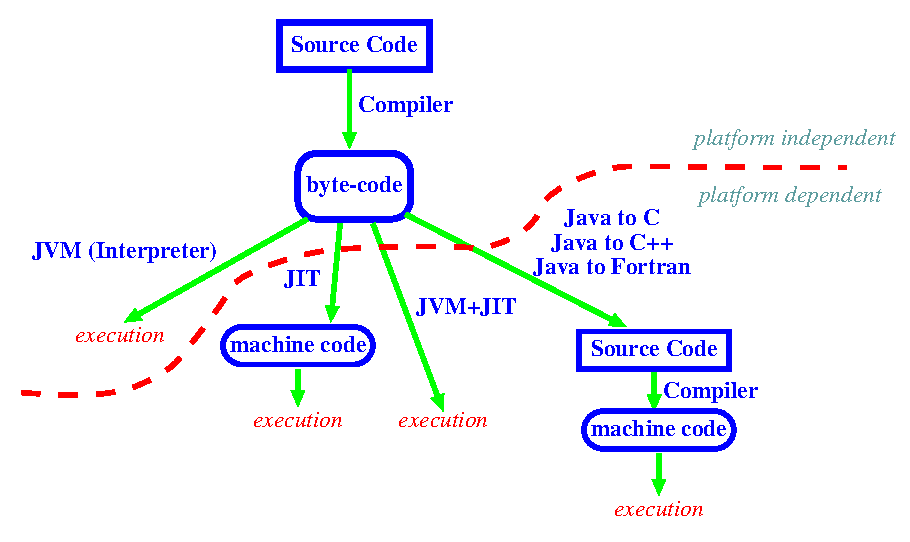
\includegraphics{Figures/Java_Overview.eps}
    \caption{Overview of the Javav language execution model.}
    \label{fig:Java_Overview}
  \end{center}
\end{figure}

So for every platform, where a virtual machine is available,
you can execute the bytecode without any compatability problems.
But the ``look and feel'' can be different, for example Java buttons
in Windows look different from buttons in X11/Motif using a UNIX
operating system. The main reason for the wide availability of Java
is that SUN Microsystems distributes the Java Development Kit (JDK)
freely for a number of important platforms (Windows, Solaris/Linux,
other Unix systems). The JDK consists of a compiler (javac), a
debugger (jdb) and a virtual machine (java)\footnote{Actually there
are some more components like the javadoc command to create HTML
documentation or the jar tool to create zipped packages of
class files belonging together - see later on.}.

The JDK can be downloaded from the internet from the 
\href{http://www.javasoft.com}{JDK Javasoft link page}.
The newest version (as of the time of writing) is 1.1.7 and is
referred to by Java 1.1. There is already a beta version for the JDK
of the new Java 1.2 language specification. Throughout the book,
we will use the Java 1.1 version and JDK 1.1.7.

The only additional thing necessary to have a Java programming
environment is an text-editor to write the Java programs. For that
you should use your favorite editor, e.g. emacs or xemacs, which are
also freely available and have nice Java editing modes.

FreeBuilder ?????

Opposing to other labguages, which use the ASCII character set, Java
uses the Unicode character set. Unicode consists of characters represented
by 2 bytes instead of 1 byte like in the ASCII set. So you can not only
use 256 different characters (ASCII) you can use all the 65535 different
characters available in the Unicode set. for writing a Java program.
This means you can name your variables using for example japanese or greek
characters. Right from the beginning, Java is an international language.

Java is also case sensitive and doesn't need any special characters
to mark continuation lines. Comments are used just like in C and C++.
You can use either the /* \ldots */ syntax (borrowed from C) for
multiline comments or the // syntax (borrowed from C++) for single
line comments. Additionally you can use /** \ldots */ for comments
to automatically generate a HTML documentation file for the class
defined in the file.
 
\subsection{The "HelloWorld" Program}
\label{sec:HelloWorld}
Now let's start with the traditional ``Hello World'' program written
in Java.

\subsubsection{Application}

\inputlisting{Listings_Java/HelloWorld_Application.java}
To execute the example you have to proceed as follows:
\begin{itemize}
\item \marginpar[Compiler]{Compiler}
        \verb/javac HelloWorld.java/  $\Longrightarrow$ produces
        HelloWorld.class in the same directory.
\item \marginpar[JVM]{JVM}
        \verb/java HelloWorld/
\item Output on screen: \verb<Hello World !<
\end{itemize}
Explanation of Programm ???????????????????

You have just written and executed your first application written in Java.


\subsubsection{Applet}

Java offers another possibility to execute code, so called Applets.
These are (small) Java programs, which are started by a server program,
e.g. a WWW browser like Netscape Navigator\footnote{You need at least 
version 4.06 or patches for earlier versions to run Java 1.1}, 
the Internet Explorer\footnote{Seems to run Java 1.1 programs since
version 4.}(Don't),
HotJava or the appletviewer\footnote{included with the JDK.}.

The ``Hello World'' example written as an applet has the following form:
\inputlisting{Listings_Java/HelloWorld_Applet.java}
As you can see there is no main method in an applet. Instead if an applet
is started by a server, the init() method is executed first. There is also
a start() (stop()) method, which is executed if the applet becomes
visible (disappears) in the server window (e.g. by scrolling in the
Netscape Naviagtor window).

The paint() method appearing in the ``Hello World'' applet is
responsible for the visual part of the applet. It uses a canvas
(drawing area) with a size defined by the calling HTML file. In our case
this HTML file could look like:
\inputlisting{Listings_Java/HelloWorld_Applet.html}
The code parameter given in the HTML file defines the name of the applet
to be run. Because there is no init() and no start() method in our
example, the paint() method gets executed by the browser (or appletviewer).
The size of the canvas has to be given in pixels explicitly in the
HTML file.

To run the applet you can either type
\begin{itemize}
\item \verb|appletviewer  HelloWorld.html| or
\item use the following URL in the browser: \\
        \verb|PATH_TO_CLASS_AND_HTML_FILE/HelloWorld.html|
\end{itemize}


\subsection{Variables}
\label{sec:Variables}
Primitive types, Strings, Objects (see later)

\subsubsection{Parameters from the command line, from the calling html page}

\subsection{Loops, Conditional Statements and simple Arithmetics}
\label{sec:Loops}
package, import, Operators +=,-=,++,\%, \&\&, ||, break,
do while, while, switch, for

Example: Mean of Random numbers

\subsection{Arrays}
\label{sec:Arrays}
allokieren, instanzieren, multidimensional arrays

Example: Mean using arrays

\subsection{Classes and Objects}
\label{sec:Classes_and_Objects}
Examples: Random Number, Moment Calculation

\inputlisting{Listings_Java/RandomNumber.java}
\inputlisting{Listings_Java/UseRandomNumber.java}

\subsubsection{Standard Mathematical Functions and mathematical libraries}
\label{sec:Standard_Math}
Math, JNL, JNT  

%%%%%%%%%%%%%%%%%%%%%%%%%%%%%%%%%%%%%%%%%%%%%%%%%%%%%%%%%%%%%%%%%
\section{More Advanced Features}

\subsection{Input/Output}
\label{sec:Input/Output}
Exception Handling, Gnuplot

\subsection{Graphics and Visualization}
\label{sec:Graphics_and_Visualization}
AWT, Graphics

Example: Random Points

Plotting using: Graph2D, Scivis,


\subsection{More Features}
\label{sec:features}
Beans, EPS Output,

\subsection{Online References}
\label{sec:Online_Refernces}


%%%%%%%%%%%%%%%%%%%%%%%%%%%%%%%%%%%%%%%%%%%%%%%%%%%%%%%%%%%%%%%%%
\section{Exercises}
radioactive decay, Pi Calc, e calc.

%%%%%%%%%%%%%%%%%%%%%%%%%%%%%%%


\bibliographystyle{peter}
\bibliography{V_98,simulit}

\selectlisting{matlab}
